\section{Dataset}
We build on dataset that was used in \cite{gkotsis2017characterisation} where they analyse textual content for the root posts in a Subreddit called Suicide Watch\footnote{\url{https://www.reddit.com/r/SuicideWatch/}}. The dataset contains a dump of 53 thousand posts from the suicide watch sub-reddit. 
However the dataset did not contain the threaded conversations for each thread. Reddit is a platform where a user can create a post on a sub-reddit, to which several members of a given sub-reddit can interact with. The array of interactions may range from simple up or down votes or posting at different hierarchy of the thread. This creates a heirarchical threaded structure of posts where the conversations end up organized like a repetetive tree structure. To understand the deeper nature of these posts,  we crawl Reddit to get the threaded conversations\footnote{The code to crawl reddit for threads can be found at \textit{https://github.com/sagarjoglekar/redditTools}} 

To baseline our work and compare theorised supportive nature of conversations with the broader community, we also crawl other subreddits like r/AskScience\footnote{\url{https://www.reddit.com/r/AskScience/}}, r/TheDonald \footnote{\url{https://www.reddit.com/r/thedonald/}} and r/ChangeMyView\footnote{\url{https://www.reddit.com/r/changemyview/}} and finally the reddit frontpage for 1 week. We acquire roughly 50 thousand baseline posts which have been popular enough to land on the front page \footnote{The reddit front page algorithm is a combination of popularity and decay in popularity as a function of time. More can be found here \url{https://goo.gl/uVdHjn}}

Figure\ref{fig:responseDist} shows the CDF for the number of responses a Root post gets on a thread across the whole dataset. 
\begin{figure}[!htb]
	\centering
	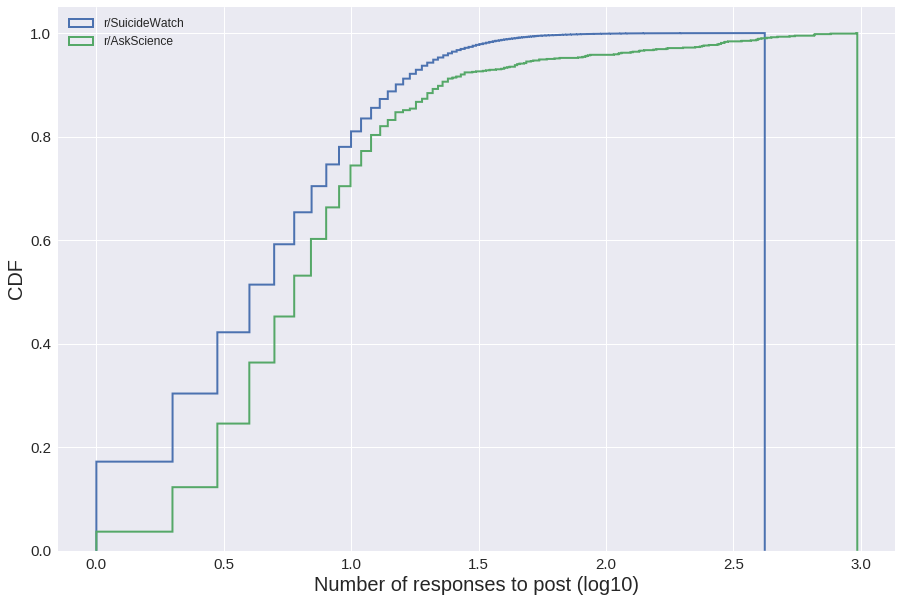
\includegraphics[width=0.5\columnwidth]{Figures/responseDistSW}
	\caption{\textsl{ Distribution of responses per thread on Subreddits r/SuicideWatch and r/AskScience }}
	\label{fig:responseDist}
\end{figure}

Figure \ref{fig:responseDist} shows the CDF for number of comments per thread across the r/SuicideWatch subreddit dataset. For comparison we show another moderated subreddit called r/AskScience. The SW sub-reddit has a Median of 4 comments per thread and a mean of 7 comments. In comparison the r/AskScience data has a median 5 comments per thread and mean of 22 comments per thread.